\graphicspath{{chapters/notes/10/images/}}
\chapter{Epigenetic profiling of cell-free DNA}

\section{Introduction}

    \subsection{Epigenetic}
    All the cells of the human organism present the same genetic information but they give rise to different types of tissues and cells.
    This happens mostly thanks to epigenetics.

        \subsubsection{Epigenetic modifications}
        The main epigenetic modifications are:

        \begin{multicols}{2}
            \begin{itemize}
                \item DNA methylation: in humans they are mainly found on CpG islands, genomic regions with high CG content.
                \item Histone post translational modifications like PTMs.
                \item chromatine architecture changes.
            \end{itemize}
        \end{multicols}

        \subsubsection{Epigenetic plasticity}
        The epigenetic landscape is very different from the genetic one.
        DNA mutations are directional: they cannot be reverted so they accumulate with subsequent cells generations.
        The epigenome is plastic, so it can be reverted, physiologically or through therapies.
        Moreover, the human epigenome is tissue and cell specific while the genome is unique.

        \subsubsection{Epigenetic deregulation}
        All levels of epigenetic controls are often deregulated in cancer: these variations usually go in favour of cancer cells survival.
        For this reason, epigenetic reprogramming has recently been added to the hallmarks of cancer.

    \subsection{DNA methylation}
    DNA methylation is the addition of methyl-groups to cytosines in CpG islands.
    It is regulated by enzymes that are responsible for regulating the cell-specific transcriptional state.
    These regulating enzymes can be:

    \begin{multicols}{2}
        \begin{itemize}
            \item Cis-factors: local control.
            \item Trans-factors: genome-wise control.
        \end{itemize}
    \end{multicols}



        \subsubsection{CpG islands}
        CpG islands are spread through the genome and when they are in a promoter they regulate gene expression through transcriptional silencing of the corresponding gene if they are methylated.
        The mechanisms are multiple and still not completely clear: DNA methylation could for example impair the binding of transcription factors or recruit repressing proteins.

        \subsubsection{Cancer tissues}
        In cancer tissue, hypomethylated and hypermethylated regions are often observed, leading to an abnormal regulation of gene expression.
        In addition to that, hypermethylation of pericentrometric heterochromatin in cancer can lead to mitotic recombination and thus genomic instability.
        Figure \ref{fig:met-cancer} depicts methylation patterns that are altered in cancer.

        \begin{figure}[H]
        \centering
            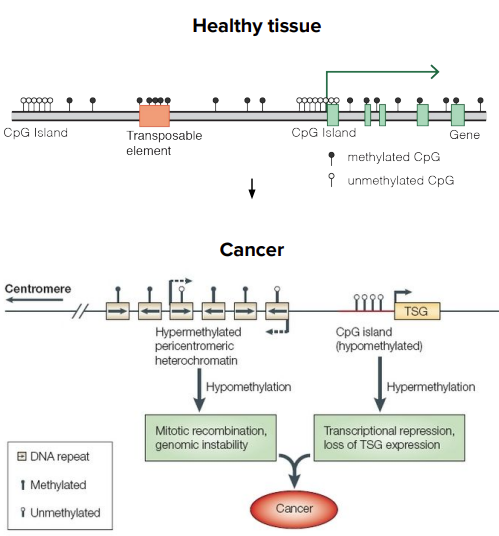
\includegraphics[width=0.5\linewidth]{cancerMet.png}
            \caption{Methylation patterns altered in cancer}
            \label{fig:met-cancer}
        \end{figure}

        \subsubsection{Landscape of regulation}
        This methylation landscape is highly regulated and tissue-specific.
        This landscape of regulation is very complex: DNA methylation can regulate gene expression but it is not the only regulating factor, some histone modifications also contribute for example.
        DNA methylations are not inherited across generations, so there is no accumulation of methylation variants, as it happens with regular DNA mutations.
        Each individual is born with a brand new methylation landscape that is then disrupted during life, not only due to cancer or disease.
        Interestingly, it could be possible to exploit variations in the DNA methylome to measure age by computing how many cell divisions led to that specific methylation state.

        \subsubsection{DNA methylation markers}
        DNA methylation markers can be:

        \begin{multicols}{2}
            \begin{itemize}
                \item Aspecific: comprising most of the genome.
                \item Tissue-specific: methylations that regulate gene expression to activate the tissue-specific functions of cells.
                \item Disease-specific: CpG hypermethylation, genome-wide hypomethylation and other modifications usually correlated with cancer.
                \item Tissue and cancer-specific: methylation patterns specific of cancer in a certain tissue.
                    These markers allow to discriminate between different tumour types.
            \end{itemize}
        \end{multicols}

    \subsection{Measuring DNA methylation}
    Figure \ref{fig:met-measure} depicts the main methods for DNA methylation measurements.
    Immunoprecipitation-based methods are also available, but the most frequently used methods are based on whole genome profiling.

\begin{figure}[H]
\centering
    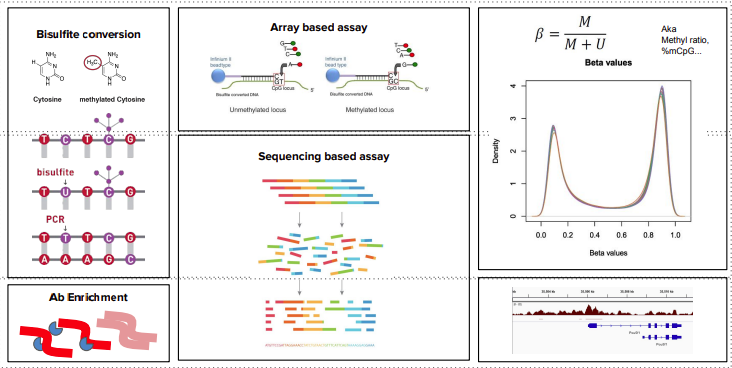
\includegraphics[width=0.8\linewidth]{methods.png}
    \caption{Main methods for DNA methylation measurement}
    \label{fig:met-measure}
\end{figure}

        \subsubsection{Bisulphite conversion}
        The fist step is to perform bisulfite conversion on DNA: thanks to bisulfate ions, unmethylated Cs are converted into Us.


        \subsubsection{Sequencing and alignment}
        The DNA so modified is then sequenced and aligned.
        The alignment is done through a particular alignment algorithm aware of the bisulfite conversion.
        In this way errors and methylations can be detected.
        Both array-based and shotgun-sequencing-based assays are used to this aim.

        \subsubsection{Computing beta values}
        The result of this assay is a series of \textbf{beta values}.
        These represent the fraction of reads corresponding to $1$ methylated genome site.

        \subsubsection{Single read analysis}
        It is useful to analyse the sequencing result at the single-read level: different methylation configurations can lead to the same global methylation level but have different biological interpretations.
        For example, a methylation level of $0.5$ can be the result of one completely methylated allele with the other one unmethylated or two half-methylated alleles.
        This kind of information is important in order to determine, for example, if the sample contains different types of cells or if it there is some disrupting pathological situation.

\section{DNA methylation based liquid biopsy}

    \subsection{Introduction}
    When a cancer cell dies, its DNA is released in circulation and it is possible to retrieve it with a liquid biopsy.
    The goal of DNA methylation-based liquid biopsies is to analyse methylations of cfDNA to retrieve information about the state of the patient, and possibly detect early-stage tumors.

    \subsection{Comparison with genomics-based liquid biopsies}
    For this purpose, when compared to genomic DNA, the analysis of the methylation landscape has positive and negative aspects.
    For genomic DNA, the percentage of actually informative signal on the whole information that is obtained can be small and difficult to observe, on the other hand, for DNA methylations it is difficult to discriminate between what is aberrant and what is not because the modifications are tissue-specific and it is difficult to obtain clear background references to make a comparison.
    A comparison of the advantages and limitation of both approaches is depicted in figure \ref{fig:comp}.

    \begin{figure}[H]
    \centering
        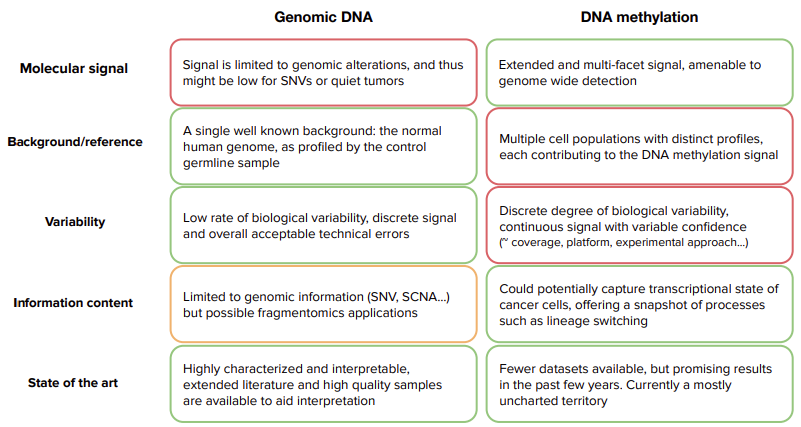
\includegraphics[width=\linewidth]{comp.png}
        \caption{\label{fig:comp}Comparison of genomics and methylation analysis for cancer detection}
    \end{figure}

    \subsection{Workflow}
    A common analysis workflow for DNA methylation based liquid biopsies is depicted in figure \ref{fig:wo}.

    \begin{figure}[H]
    \centering
        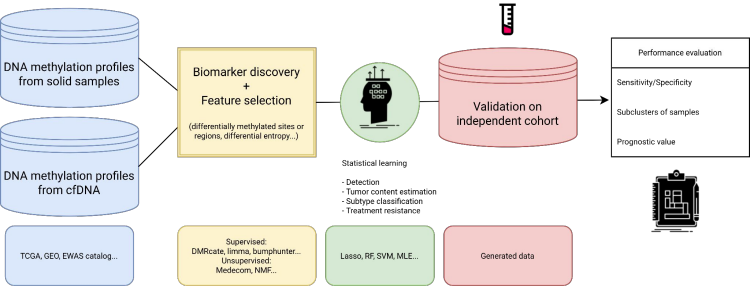
\includegraphics[width=0.8\linewidth]{workflow.png}
        \caption{Common DNA methylation based liquid biopsies analysis workflow}
        \label{fig:wo}
    \end{figure}

    Different steps in the workflow can be identified:

    \begin{multicols}{2}
        \begin{enumerate}
            \item The data is sequenced from solid and liquid samples because the methylation profiles from solid samples are needed as reference.
                The reference profiles for liquid biopsies analysis are derived from white blood cells and from the cancer type of interest.
                White blood cells are the background reference for cfDNA, since the most frequent genomic material in circulation originates from this type of cells.
            \item If a methylation pattern different from the one of blood cells is found in cfDNA it means that cells of some other tissue are dying and their material is going into circulation.
                This is a possible signal of disease.
            \item Once having obtained these reference pattern, biomarkers are searched and feature selection is performed.
            \item A model is fitted and optimized to perform predictions on new data.
            \item Performance evaluation of the model is done.
        \end{enumerate}
    \end{multicols}

    \subsection{CCGA study}
    The Circulating Cell-free Genome Atlas (CCGA) is a study conducted by Grail designed to characterize the landscape of genomic cancer signals in the blood of people with and without cancer.
    The study enrolled approximately $15000$ participants.
    Their goal is early and simple detection of cancer from analysis of methylations on cell-free DNA.

        \subsubsection{Obtaining methylation profiles}
        They performed whole genome methylation profiles after choosing between three different independent methods:

        \begin{multicols}{2}
            \begin{itemize}
                \item Whole genome sequencing.
                \item Targeted sequencing.
                \item Whole genome sequencing for CNVs.
            \end{itemize}
        \end{multicols}

        In the second phase an assay for a targeted methylation study has been developed: the best features to discriminate between the two classes (cancer vs non-cancer) were selected in order to sequence the areas with these modifications without whole genome analysis.
        A model for this classification was developed, trained and validated.
        The last step is a large-scale clinical validation with a $5$ years follow-up that is still in progress.

        \subsubsection{Results}
        This process had good results but not for all cancer types: sensitivity is better for cancers of highly-vasculated tissues and metastatic tumors, while some types of cancer produce a lot of false negative results.
        Moreover, detection is obviously better when cancer progresses but the goal is early detection.

    \subsection{Deconvolution approach}
    Deconvolution of cell-free DNA is another task to be performed on DNA methylation other than classification.
    The goal is to explain the observed signal with a combination of pure signals: discover the main contribution that led to a specific methylation landscape.
    One example of this is tumour profiling.

        \subsubsection{Considering liquid biopsies}
        From liquid biopsies, it is possible to detect which are the main contributors to the cfDNA.
        These results can be compared with the ones obtained from cancer patients to determine which are the contributors to the difference in cfDNA that is observed and to infer data for tumour diagnosis or treatment resistance detection.

        \subsubsection{High-quality reference atlases}
        In order to perform deconvolution, high-quality reference atlases are needed: one was built with the contribution of \href{https://www.biorxiv.org/content/10.1101/2022.01.24.477547v1}{Grail}.
        They sorted healthy donors cells with FACS and profiled them.
        Cell type specific metylation profiles were built, so it is possible to use this atlas to select biomarkers, like a reference genome.
        They generated specific methylation patterns for $39$ human cell types from $207$ methylomes.

    \subsection{Targeted panel approaches for tumour content estimation}
    The interest of this group is detection of treatment resistance in prostate cancer.
    The goal is to know when the tumour becomes resistant, in order to be able to change or calibrate the therapy.
    A sequencing panel was developed to detect the amount of cancer-derived DNA in circulation, and interestingly only $50$ regions are sufficient to get a satisfying estimation.
    A model is built to know how much ctDNA is expected after treatment and it is possible to get a score that estimates the level of resistance.
